%!TEX root=../main.tex

\appendix

\section{Heuristic Approaches}
\label{sec:heuristic}
% %!TEX root = ../main.tex

\subsection{A plausible (but bad) alternative}
\label{sec:dt}

% \sys analyzes query logs and complaints by producing a mathematical
% formulation of the constraints that need to be satisfied. The
% constraint problem can then be evaluated by dedicated external tools.

The MIP models generated by \sys can grow large as the sizes of the
data and the log increase. However, modeling all present constraints
from the beginning to the end of the log is necessary; in this
section, we examine alternative, simpler models that process a single
query at a time, and demonstrate why they are insufficient.

\smallskip
\noindent
\textbf{WHERE repairs through classification:}
The \texttt{WHERE} clause of an update query is equivalent to a
rule-based binary classifier that splits tuples into two groups:
(1)~tuples that satisfy the conditions in the \texttt{WHERE} clause
and (2)~tuples that do not. A mistake in a query predicate can then
result in misclassification: some tuples get classified into the wrong
group, which in turn translates to errors in the data. Therefore,
repairing the mistake corresponds to repairing the imprecise
classification. This works as follows: For an incorrect query $q$, let
$D_0$ be the database state before $q$, and $D_1^*$ the \emph{correct}
database state that should result after $q$.
We use each tuple $t \in D_0$ as an element in the input training data
for the classifier where the values (of each attribute) of $t$ define
the feature vector and the label for $t$:
	\[
    label(t)= 
    \begin{cases}
    true ,& D_0.t \neq D_1^*.t\\
    false,              & \text{otherwise}
    \end{cases}
\]
We then train a classifier, such as decision trees \cite{???} to learn
the correct classification rules rules for the \texttt{WHERE} clause.


\smallskip
\noindent
\textbf{SET repairs:}
After repairing the \texttt{WHERE} clause through learning a
rule-based classifier, some complaints may still persist. This
indicates a possible error in the \texttt{SET} clause. The errors can
be modeled and solved by constructing a simple linear system of
equations: For each expression in the \texttt{SET} clause we create a
linear equation, using unknown variables to represent any parameters
in the \texttt{SET} expression. Solving for these variables then
provides a repair for the \texttt{SET} expression.


\smallskip
\noindent
\textbf{Why it does not work:}
The na\"ive approach that we just described is heuristic in nature. It
is simple and fast, but it can only process a single incorrect query.
This results in several shortcomings that make it insufficient in
practice:
\begin{itemize}[itemsep=1pt, leftmargin=5mm]
    
\item In principle, one could attempt to apply this technique to the
entire log one-query-at-a-time. However, this is not possible in
practice: to learn a classifier on the \texttt{WHERE} clause of query
$q_i$, one needs to know the correct classification output, which
corresponds to $D_i^*$. Unfortunately, even with a complete complaint
set, which can derive the correct database $D_n^*$, there is no
obvious way to ``rollback'' this state to derive $D_i^*$.

\item The classifier may derive a clause that is structurally very
different from the original one (different attributes or number of
conditions). This is problematic in general, as it corresponds to a
larger-scale mistake in the query, which is a less likely scenario.

\item Classifiers try to avoid overfitting, which is problematic for
queries with high selectivity (e.g., single-tuple updates), as the
classifier is unlikely to generate any rules.

\end{itemize}


Therefore, while examining one query at a time superficially appears
to be a reasonable and efficient alternative, the reality is that one
has to model all constraints and transformations through the entire
log history. In the following section, we propose several
optimizations to our initial approach that make scaling to large data
and log sizes feasible. 
% \red{Add graph comparing naive and d-trees here.}


\iffalse
In this
section, we examine alternative, simpler models that process a single
query at a time, and demonstrate why they are insufficient.

\noindent
\textbf{WHERE repairs through classification:}
The \texttt{WHERE} clause of an update query is equivalent to a
rule-based binary classifier that splits tuples into two groups:
(1)~tuples that satisfy the conditions in the \texttt{WHERE} clause
and (2)~tuples that do not. Thus, by training a classifier,
such as decision trees \cite{quinlan1987} to learn
the correct classification rules rules for the \texttt{WHERE} clause.

\noindent
\textbf{SET repairs:}
This alternative approach constructs 
a simple linear system of equations to solve the parameters in the \texttt{SET}
when errors persist after fixing the \texttt{WHERE} clause:
For each expression in the \texttt{SET} clause we create a
linear equation, using unknown variables to represent any parameters
in the \texttt{SET} expression. 
  \begin{figure}[h]
  \centering
    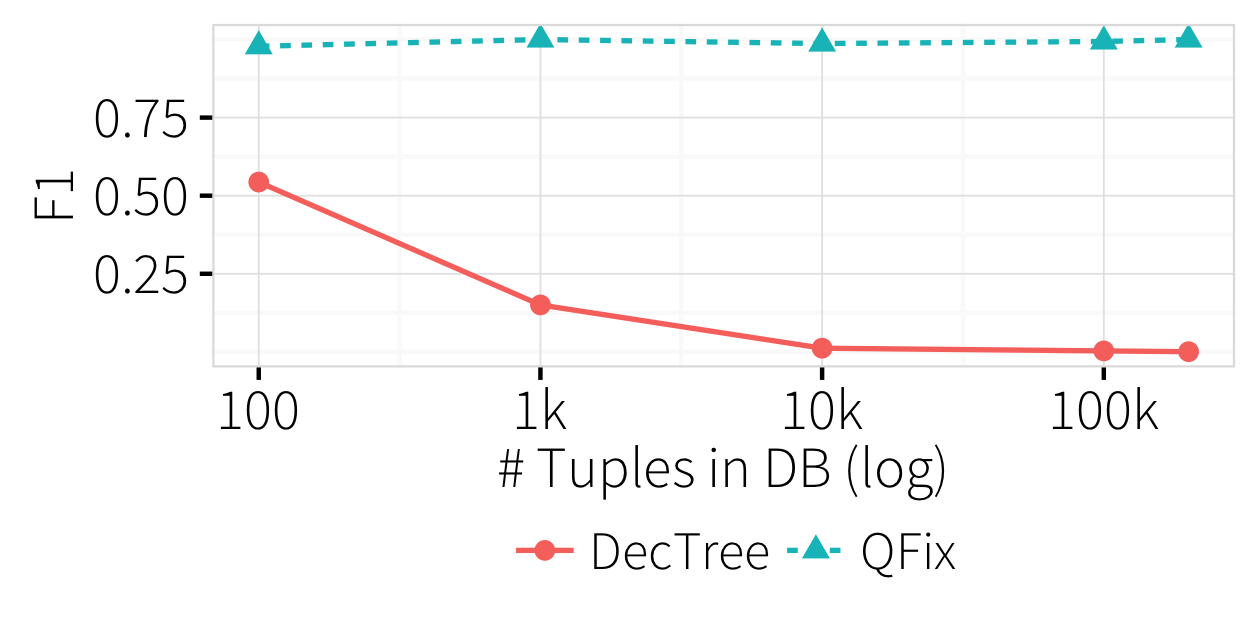
\includegraphics[width = .6\columnwidth]{figures/heuristicacc}
    \vspace*{-.1in}
    \caption{Heuristic Approach vs. \sys on Single-Query. }
    \label{f:heuristic_acc} 
  \end{figure}
  \vspace*{-0.1in}
  
The na\"ive approach that we just described is heuristic in nature. It
is simple and fast, but it can only process a single incorrect query. As shown in
Figure~\ref{f:heuristic_acc}, the F-1 score of na\"ive heuristic approach is less 
than 0.6 while \sys maintain high accuracy in solving single query problem with
above 0.9 F-1 score across all database sizes. 
\fi

The MILP models generated by \sys can grow large as the sizes of the
data and the log increase. However, modeling all present constraints
from the beginning to the end of the log is necessary; in this
section, we examine alternative, simpler models that process a single
query at a time, and demonstrate why they are insufficient 
theoretically and experimentally.
  \begin{figure*}[t]
  \centering
  \begin{subfigure} [t]{.3\textwidth}
    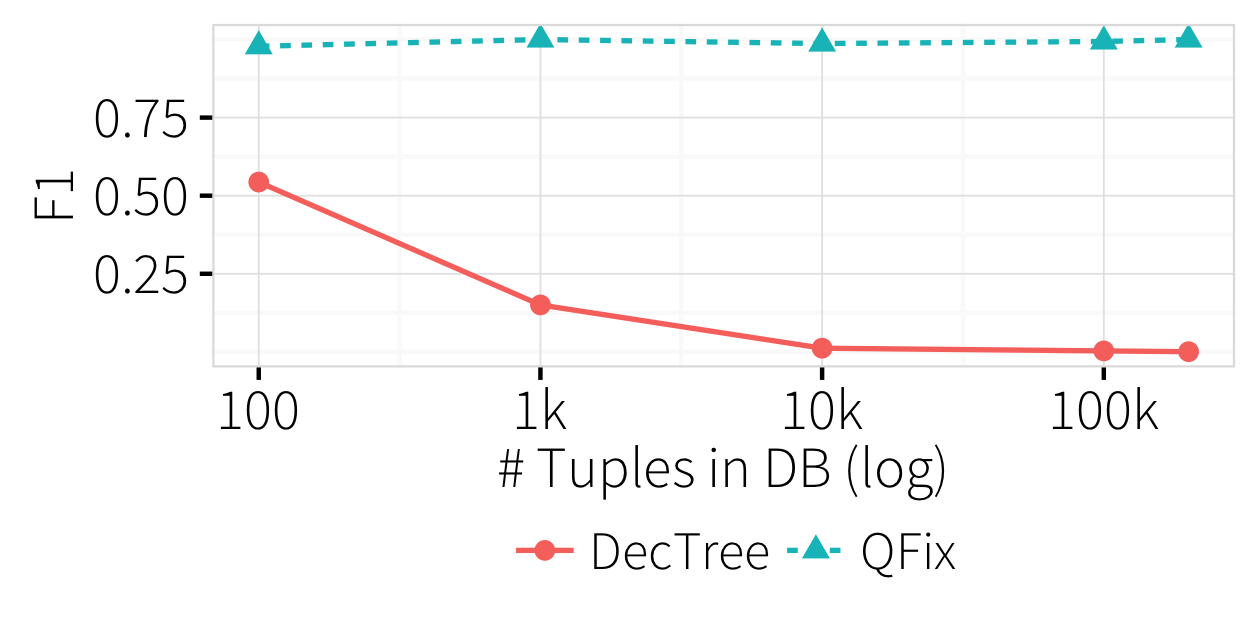
\includegraphics[width = .99\columnwidth]{figures/heuristicacc}
    \vspace*{-.25in}
    \caption{Comparison on Accuracy. }
    \vspace*{-.1in}
    \label{f:heuristic_acc} 
    \end{subfigure}
      \begin{subfigure} [t]{.3\textwidth}
    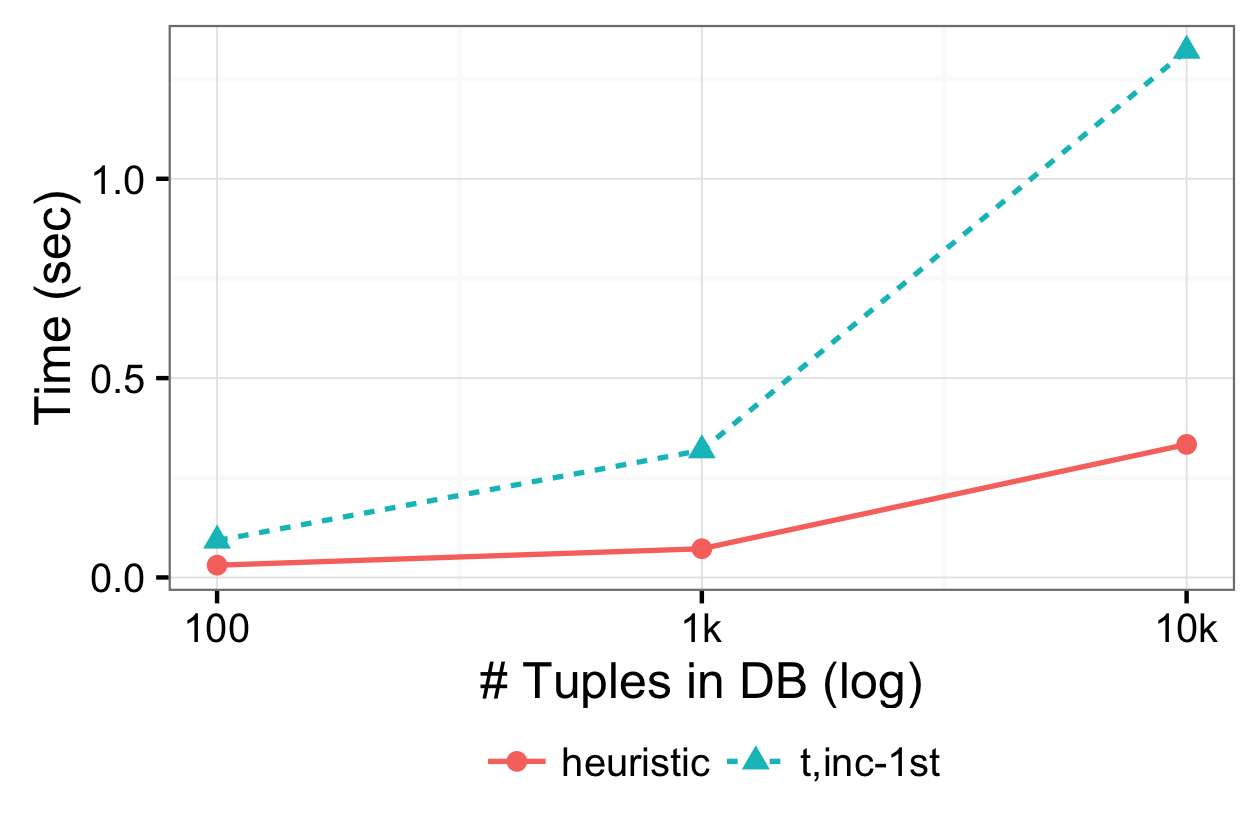
\includegraphics[width = .99\columnwidth]{figures/heuristictime}
    \vspace*{-.25in}
    \caption{Comparison on Performance. }
    \vspace*{-.1in}
    \label{f:heuristic_time} 
    \end{subfigure}
   \caption{Heuristic Approach vs. \sys}
   \vspace*{-.1in}
  \end{figure*}
  
\smallskip
\noindent
\textbf{WHERE repairs through classification:}
The \texttt{WHERE} clause of an update query is equivalent to a
rule-based binary classifier that splits tuples into two groups:
(1)~tuples that satisfy the conditions in the \texttt{WHERE} clause
and (2)~tuples that do not. A mistake in a query predicate can then
result in misclassification: some tuples get classified into the wrong
group, which in turn translates to errors in the data. Therefore,
repairing the mistake corresponds to repairing the imprecise
classification. This works as follows: For an incorrect query $q$, let
$D_0$ be the database state before $q$, and $D_1^*$ the \emph{correct}
database state that should result after $q$.
We use each tuple $t \in D_0$ as an element in the input training data
for the classifier where the values (of each attribute) of $t$ define
the feature vector and the label for $t$:
	\[
    label(t)= 
    \begin{cases}
    true ,& D_0.t \neq D_1^*.t\\
    false,              & \text{otherwise}
    \end{cases}
\]
We then train a rule-based classifier, 
such as decision trees \cite{quinlan1987} to learn
the correct classification rules rules for the \texttt{WHERE} clause.


\smallskip
\noindent
\textbf{SET repairs:}
After repairing the \texttt{WHERE} clause through learning the classifier, 
some complaints may still persist. This
indicates a possible error in the \texttt{SET} clause. The errors can
be modeled and solved by constructing a simple linear system of
equations: For each expression in the \texttt{SET} clause we create a
linear equation, using unknown variables to represent any parameters
in the \texttt{SET} expression. Solving for these variables then
provides a repair for the \texttt{SET} expression.


\smallskip
\noindent
\textbf{Why it does not work:}
The approach that we just described is heuristic in nature. It
is simple and fast, but it can only process a single incorrect query.
This results in several shortcomings that make it insufficient in
practice:
\begin{itemize}[itemsep=1pt, leftmargin=5mm]
    
\item \textbf{Single Query Limitation: }
In principle, one could attempt to apply this technique to the
entire log one-query-at-a-time. However, this is not possible in
practice: to learn a classifier on the \texttt{WHERE} clause of query
$q_i$, one needs to know the correct classification output, which
corresponds to $D_i^*$. Unfortunately, even with a complete complaint
set, which can derive the correct database $D_n^*$, there is no
obvious way to ``rollback'' this state to derive $D_i^*$.

\item \textbf{Different Query Structure: } 
The classifier may derive a clause that is structurally very
different from the original one (different attributes or number of
conditions). This is problematic in general, as it corresponds to a
larger-scale mistake in the query, which is a less likely scenario.

\item \textbf{Low Precision: }
Classifiers try to avoid overfitting, which is problematic for
queries with high selectivity (e.g., single-tuple updates), as the
classifier is unlikely to generate any rules.
\end{itemize}

To illustrate these shortcomings, we compare this heuristic approach and the \sys approach
using our synthetic data generator with increasing database size 
and single query logs. As shown in Figure~\ref{f:heuristic_acc}, the heuristic approach
is more efficient than \sys, however, its
F1-scores are constantly below 0.5 across
different database sizes where as \sys maintain above 0.9 accuracy. \\
Therefore, while examining one query at a time by  
superficially appears
to be a reasonable and efficient alternative, 
the reality is that one
has to model all constraints and transformations through the entire
log history. In addition, even with single query, though more efficient than \sys, 
the heuristic alternative can hardly achieve near satisfiable accuracy. 

\iffalse
In this
section, we examine alternative, simpler models that process a single
query at a time, and demonstrate why they are insufficient.

\noindent
\textbf{WHERE repairs through classification:}
The \texttt{WHERE} clause of an update query is equivalent to a
rule-based binary classifier that splits tuples into two groups:
(1)~tuples that satisfy the conditions in the \texttt{WHERE} clause
and (2)~tuples that do not. Thus, by training a classifier,
such as decision trees \cite{quinlan1987} to learn
the correct classification rules rules for the \texttt{WHERE} clause.

\noindent
\textbf{SET repairs:}
This alternative approach constructs 
a simple linear system of equations to solve the parameters in the \texttt{SET}
when errors persist after fixing the \texttt{WHERE} clause:
For each expression in the \texttt{SET} clause we create a
linear equation, using unknown variables to represent any parameters
in the \texttt{SET} expression. 
  \begin{figure}[h]
  \centering
    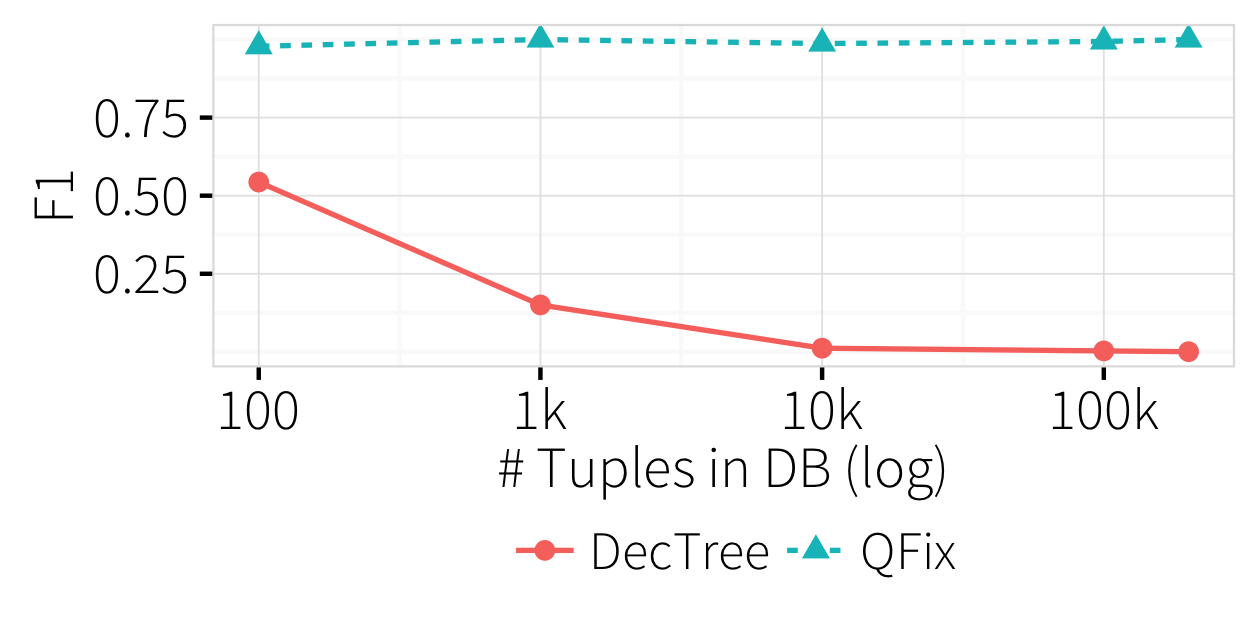
\includegraphics[width = .6\columnwidth]{figures/heuristicacc}
    \vspace*{-.1in}
    \caption{Heuristic Approach vs. \sys on Single-Query. }
    \label{f:heuristic_acc} 
  \end{figure}
  \vspace*{-0.1in}
  
The na\"ive approach that we just described is heuristic in nature. It
is simple and fast, but it can only process a single incorrect query. As shown in
Figure~\ref{f:heuristic_acc}, the F-1 score of na\"ive heuristic approach is less 
than 0.6 while \sys maintain high accuracy in solving single query problem with
above 0.9 F-1 score across all database sizes. 
\fi
  
\section{Effect of Index of Corrupted Query}
\label{app:qidx}

A key parameter for our experiments is the location of the corrupted query ($idx$).  
\alex{Have we discussed anywhere yet that we focus on single errors?}
This parameter determines the number of queries \sys must consider when searching for a fix,
and affects the size of the complaint set.  
\alex{It won't be clear to the reader how this relates to the size of the complaint set.}
Both of these characteristics directly impact \sys's 
runtime performance. For this reason, it is undesirable to randomly pick and corrupt queries
throughout the query log, as the performance and accuracy results may not be comparable. 
To better understand the relationship between $idx$ and the size of the complaint set, we ran
simulations using a database with $20$ attributes, and a query log of size $1000$ containing
either all $set = const$ or $set = rel$ \texttt{UPDATE} queries.
We varied  $idx$ uniformly throughout the query log, and additionally varied
the skew $s$ and range $r$ parameters to study how they affect the size of the complaint sets.


  \begin{figure}[h]
  \centering
  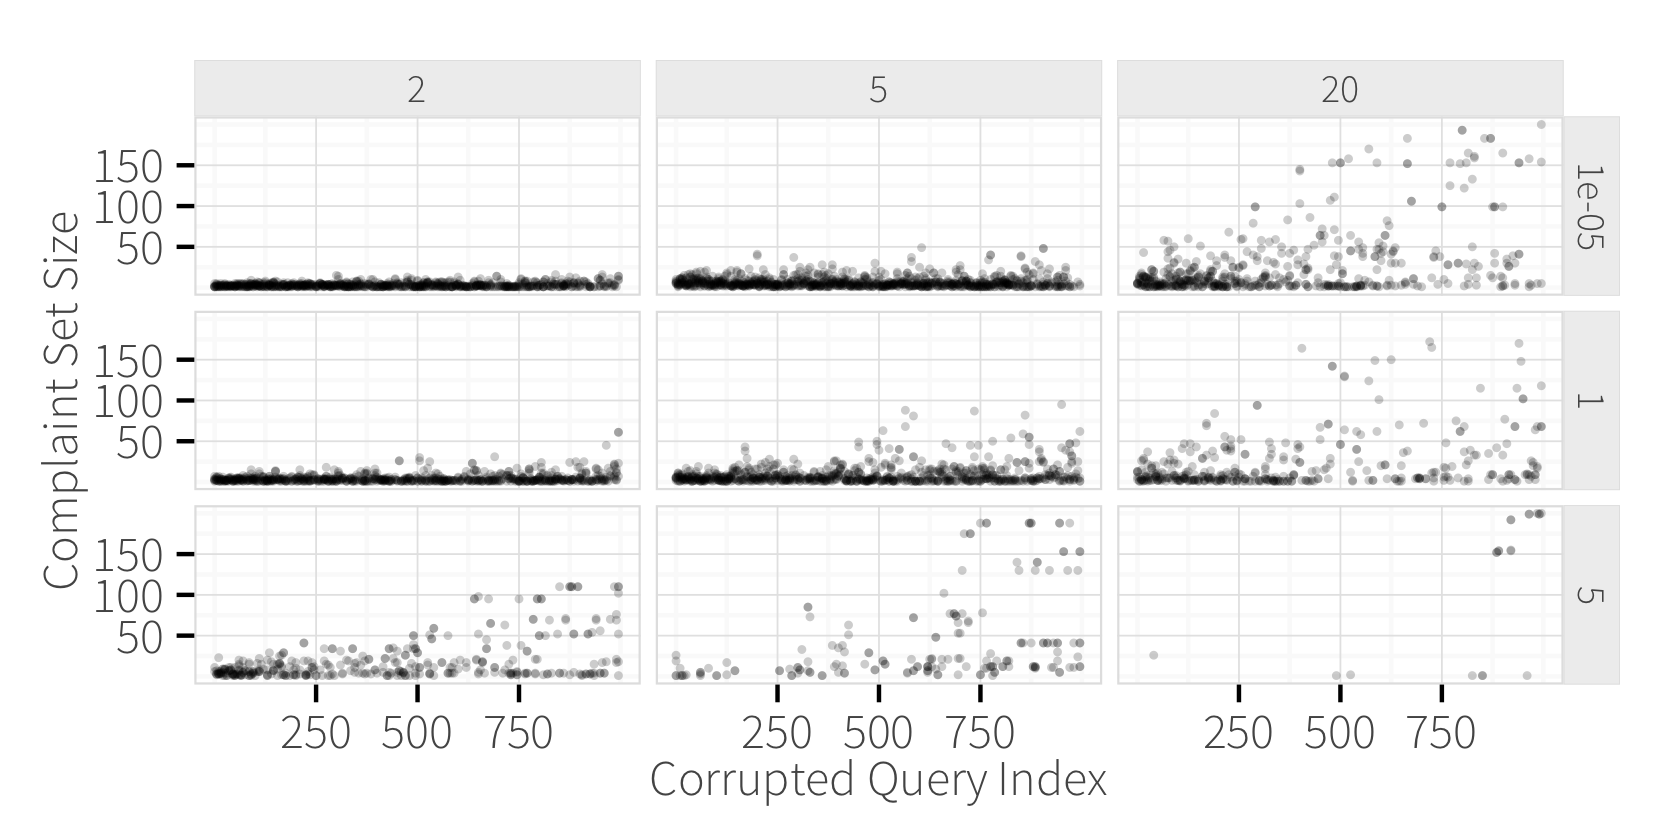
\includegraphics[width = 3.5in]{figures/qidxsimulation/qidx_v_ncomplaints_20attrs_const}
  \caption{Query index vs complaint set size for $set = const$.}
  \label{f:qidx_v_ncomplaints_const} 
  \end{figure}


Figure~\ref{f:qidx_v_ncomplaints_const} plots a representative set of parameters.  We plot one point
for each corrupted query index that results in a complaint set with at least one complaint. 
These results highlight several interesting trends.  When queries do not overlap ($r = 1$, leftmost column),
the size of the complaint sets are relatively small, and their frequency is constant across the possible query indices.
However as the possibility of overlap increases (e.g., $r$ increases), more recent queries are more likely to result in
very large complaint sets (at times the size of the database).   
This effect is a symptom of the fact that queries with large ranges will set groups of tuples to the same value,
and over time, skew the distribution of tuple values to a small number of possible values.
Thus, more recent corruptions that affect a large cluster of similar tuples will result in a large complaint set.
We find that increasing the skew parameter also exacerbates this effect.  
In addition, high skew increases the likelihood that queries will share the same \texttt{WHERE} and \texttt{SET} clause 
attributes as a corrupted query, thus overwriting the error introduced by the corrupted query.  
This is why the frequency of non-empty complaint sets decreases significantly as $s$ increases.


\begin{figure}[h]
\centering
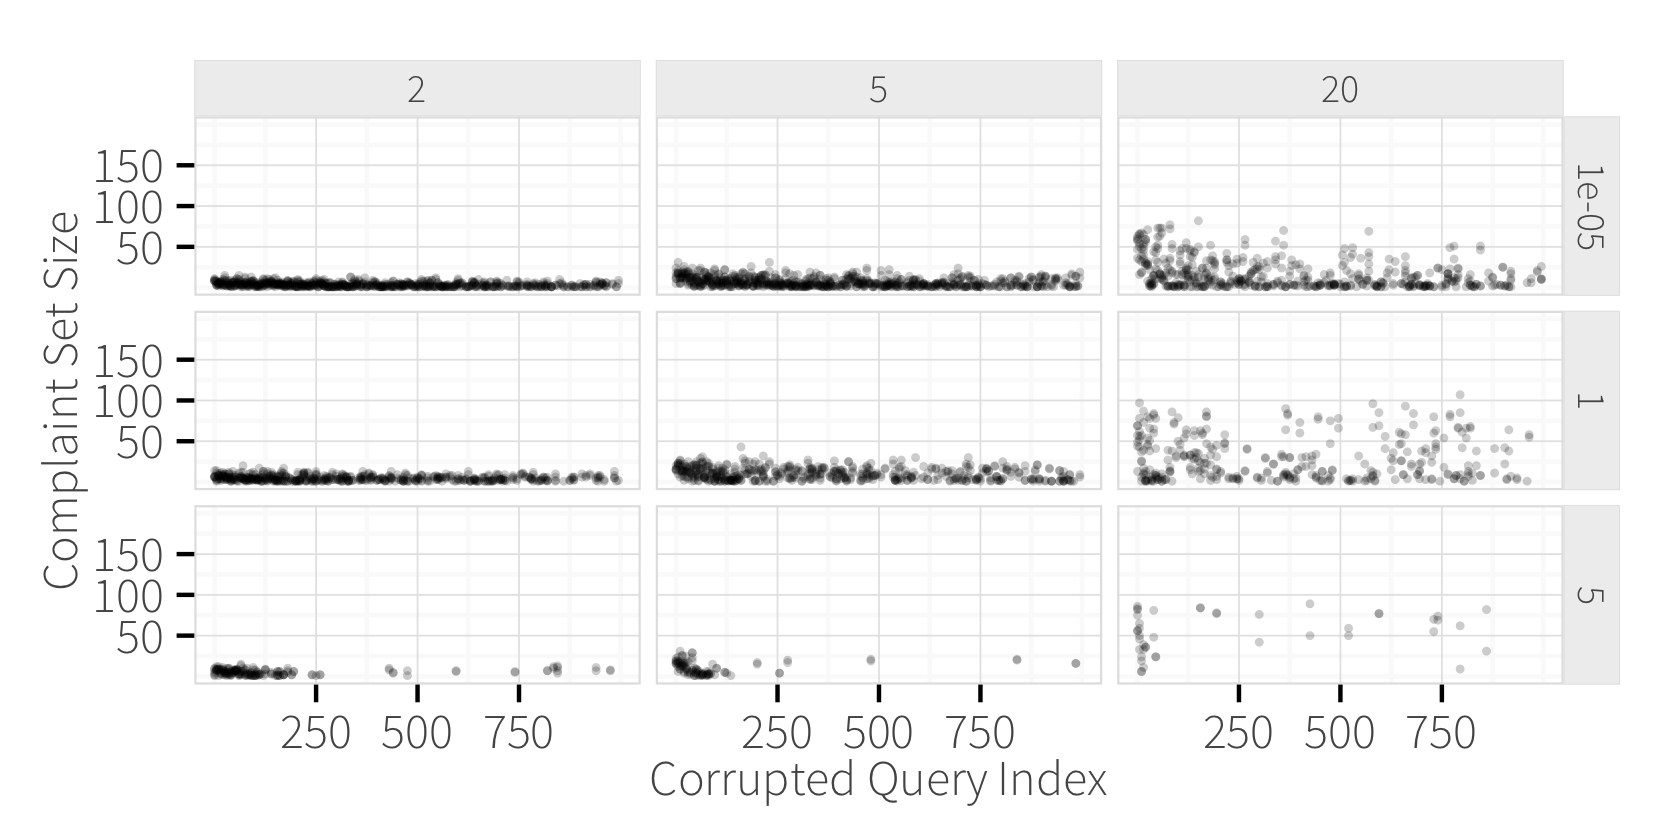
\includegraphics[width = 3.5in]{figures/qidxsimulation/qidx_v_ncomplaints_20attrs_rel}
\caption{Query index vs complaint set size for $set = rel$.}
\label{f:qidx_v_ncomplaints_rel} 
\end{figure}

In contrast to $set=const$ queries, Figure~\ref{f:qidx_v_ncomplaints_rel} executes the 
same experiment using $set=rel$ queries.  In this setting, we find that the trend is
reversed, and older corruptions tend to result in larger complaint sets.  This is because,
subsequent \texttt{UPDATE} queries increment or decrement the attribute value, rather than
overwriting it with a constant value.  The clustering of data values due to query overlap
then increases the number of other tuples affected.


\ewu{summarize findings and implications to experiments here.}
not all corruptions result in complaint sets.
In constant SET clause workloads, larger complaints sets are more likely to
result from more recent corrupted queries -- particularly if the queries are range updates or
the updated attributes are skewed.
For this reason, our experiments corrupt the query log at six positions 
$idx \in \{0, 25, 50, 100, 200, 250\}$ , relative 
to the most recent query (e.g., the most recent query, the $25^th$ most recent query, and so on).

% \begin{figure}[h]
% \centering
% 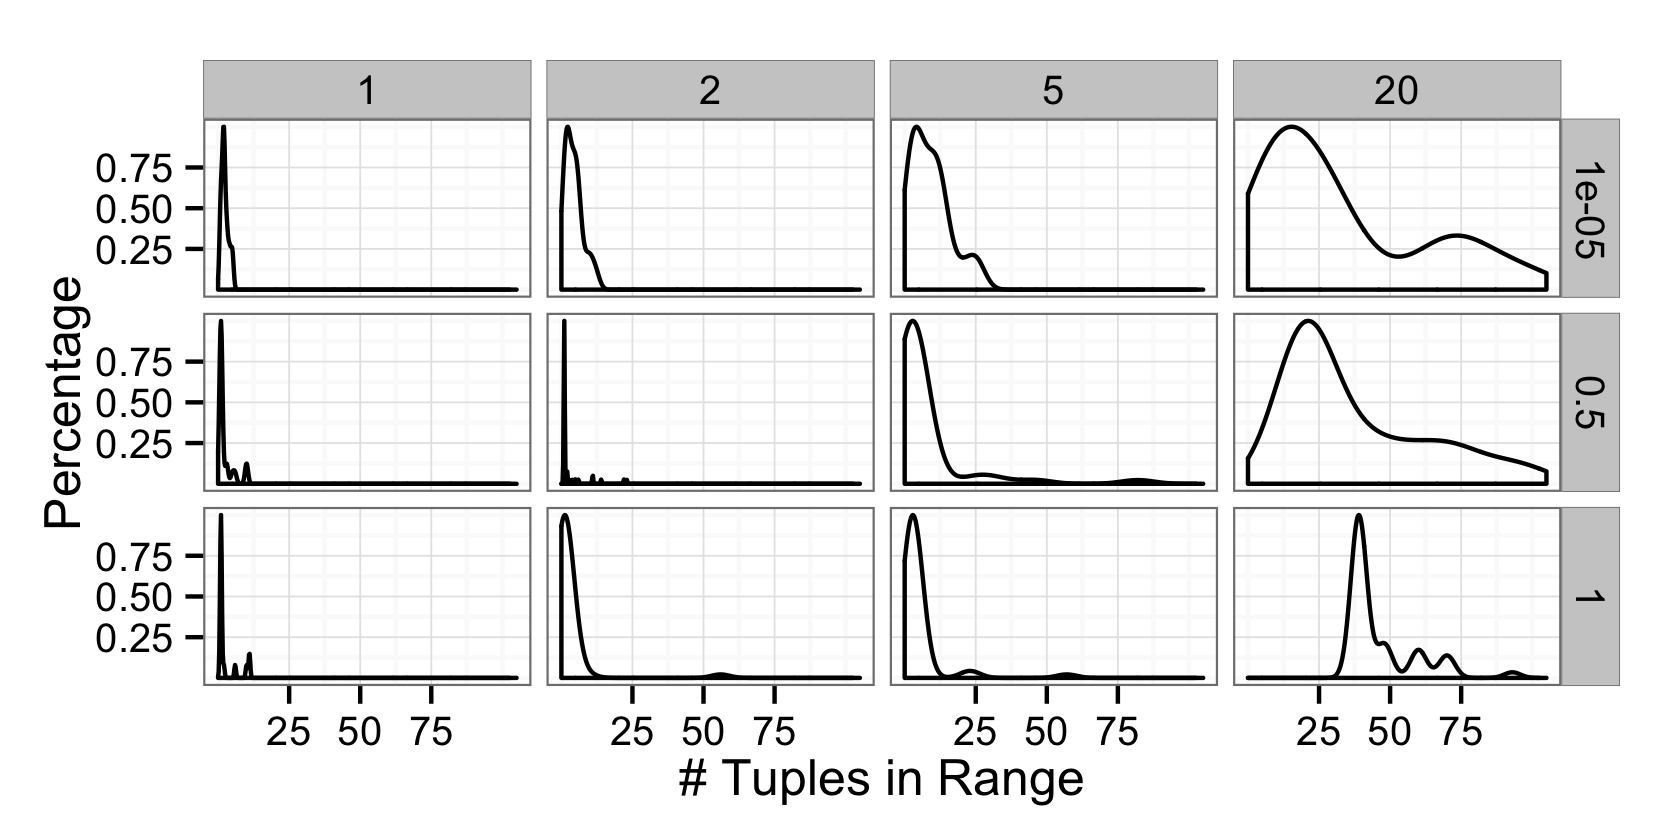
\includegraphics[width = 3.5in]{figures/qidxsimulation/numinrange}
% \caption{.}
% \label{f:numinrange} 
% \end{figure}


As we observed from Figure~\ref{f:multiquery}, \milpall maintains high accuracy when errors
happen more recent, however it does not scale when the error locate further from the most
recent query. \milptuple scales better than \milpall, but ignoring tuples not 
in the complaint set apparently hurts the precision. \milptuplestopearly run times faster
than \milpall and \milptuple, however the aggressive strategy greatly reduce the 
precision. In the end, \milpadvtuple significantly improves the precision with very limited
time cost compare to \milptuple. \\
Based on these observations, we only include the performance of \milpadvtuple and \milpadvall
in the rest of the experiments. 

\section{Solving time for the solver}
\label{app:solvtime}
